\documentclass[../../Problems]{subfiles}
\begin{document}
\subsection{L-Systems}{\label{pp:lsystems}}
Lindenmayer system, shortly L-system is a recursive system to generate self-similar patterns.
Simply put, it contains variables, constants, an axiom and rules.

In fact, we have already seen its example \hyperref[pp:thuemorsesequence]{here}. So, let's take that as a reference. We can generate the Thue-Morse Sequence using the below L-System
\begin{description}
	\item[variables] 0,1
	\item[constants] none
	\item[axiom] 0 (start with 0)
	\item[rules] 0 $\rightarrow$ 01, 1 $\rightarrow$ 10 (replace 0 by 01 in next step and 1 by 10)
\end{description}
This produces the following sequences
\begin{description}
	\item[Iterate 0] 0
	\item[Iterate 1] 01
	\item[Iterate 2] 0110
	\item[Iterate 3] 01101001
	\item[Iterate 4] 0110100110010110 and so on
\end{description}
\subsubsection{Dragon Curve}{\label{pp:dragoncurve}}
\begin{description}
	\item[variables] F,G
	\item[constants] +--
	\item[axiom] F
	\item[rules] F $\rightarrow$ F+G, G $\rightarrow$ F--G
\end{description}
The generated sequence is F+G+F--G+F+G--F--G+F+G+F--G--F+G--F--G$\ldots$. Consider F, G as moving forward and + (--) as turning left (right) by 90$^\circ$.

\textbf{Problem Statement:}\\
Draw the corresponding curve using \verb!turtleSim! with appropriate scaling such that it roughly takes same width and height for all iterates.
\begin{tcolorbox}[breakable, enhanced, sharpish corners]%, colback = white]
	\href{https://github.com/paramrathour/CS-101/tree/main/Starter Codes/Dragon Curve.cpp}{\textbf{Starter Code}}
\end{tcolorbox}
\begin{figure}[H]
	\centering
	\begin{subfigure}{0.1\linewidth}
		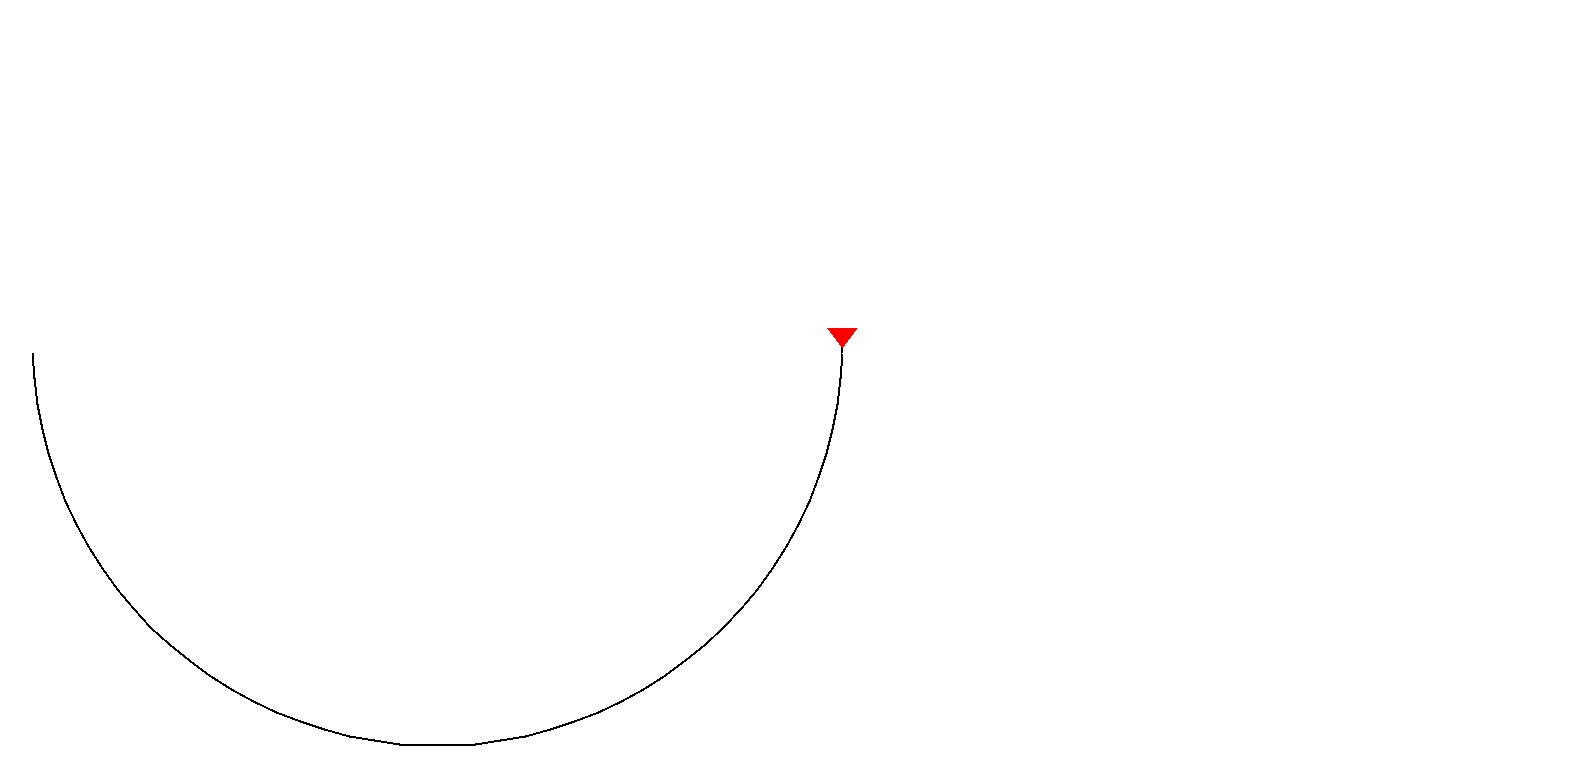
\includegraphics[width = \linewidth]{Dragon Curve/1.png}
		\caption{Iterate 1}
	\end{subfigure}
	\begin{subfigure}{0.08\linewidth}
		\includegraphics[width = \linewidth]{Dragon Curve/2.png}
		\caption{Iterate 2}
	\end{subfigure}
	\begin{subfigure}{0.12\linewidth}
		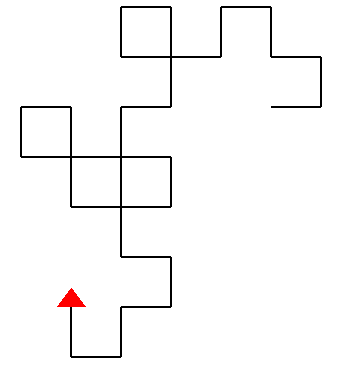
\includegraphics[width = \linewidth]{Dragon Curve/5.png}
		\caption{Iterate 5}
	\end{subfigure}
	\begin{subfigure}{0.16\linewidth}
		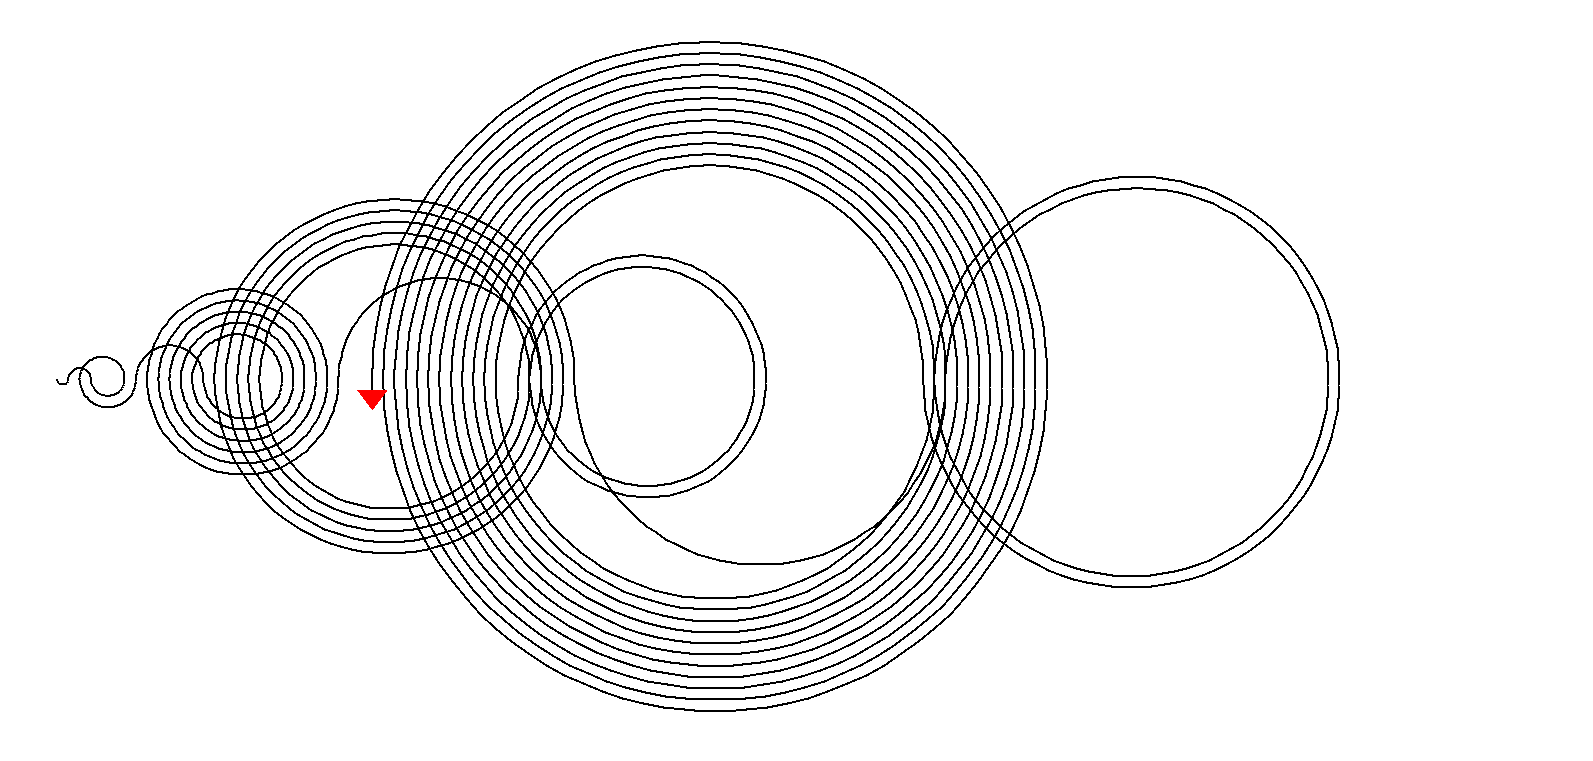
\includegraphics[width = \linewidth]{Dragon Curve/7.png}
		\caption{Iterate 7}
	\end{subfigure}
	\begin{subfigure}{0.09\linewidth}
		\includegraphics[width = \linewidth]{Dragon Curve/10.png}
		\caption{Iterate 10}
	\end{subfigure}
	\begin{subfigure}{0.18\linewidth}
		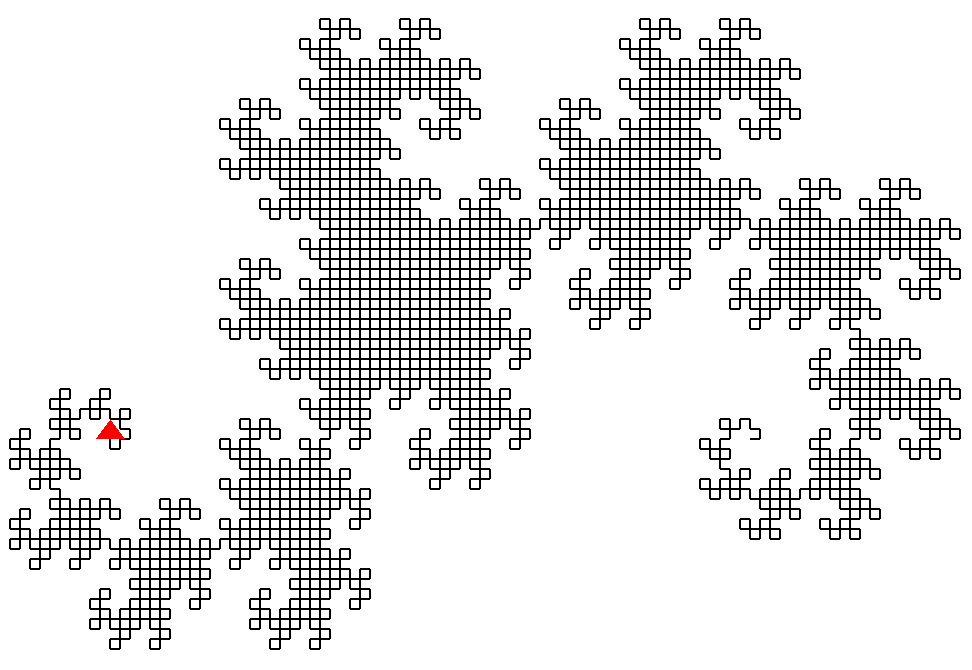
\includegraphics[width = \linewidth]{Dragon Curve/12.png}
		\caption{Iterate 12}
	\end{subfigure}
	\begin{subfigure}{0.18\linewidth}
		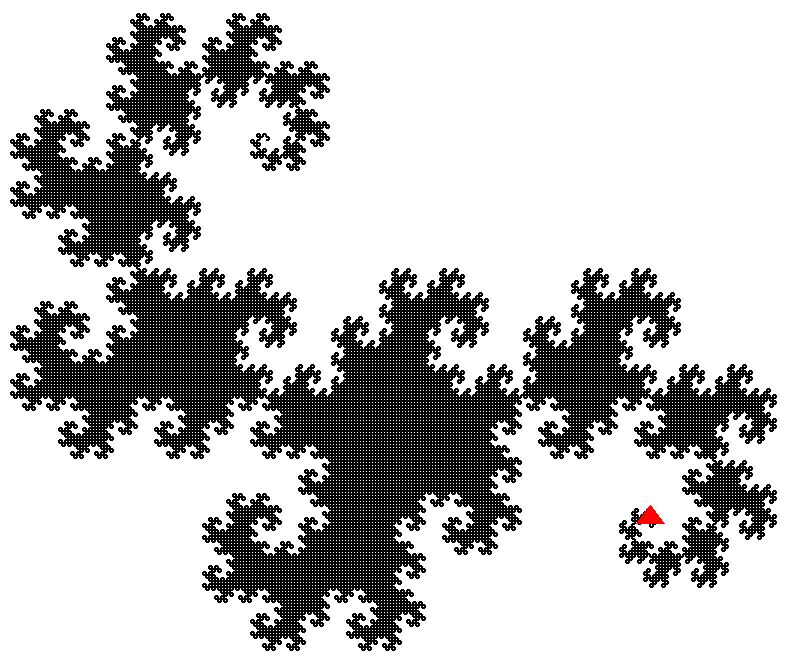
\includegraphics[width = \linewidth]{Dragon Curve/15.png}
		\caption{Iterate 15}
	\end{subfigure}
	\caption{Dragon Curve iterates}
\end{figure}
\vspace{-2em}
\subsubsection{Sierpi\'nski Arrowhead Curve}{\label{pp:sierpinskicurve}}
\begin{description}
	\item[variables] A,B
	\item[constants] +--
	\item[axiom] A
	\item[rules] A $\rightarrow$ B--A--B, B $\rightarrow$ A+B+A
\end{description}
Try generating this. Here, A, B denote moving forward and + (--) denote turning left (right) by 60$^\circ$.

\textbf{Problem Statement:}\\
Again, draw the corresponding curve using \verb!turtleSim! with appropriate scaling such that it roughly takes same width and height for all iterates.
\begin{tcolorbox}[breakable, enhanced, sharpish corners]%, colback = white]
	\href{https://github.com/paramrathour/CS-101/blob/main/Starter%20Codes/Sierpi%C5%84ski%20Arrowhead%20Curve.cpp}{\textbf{Starter Code}}
\end{tcolorbox}
\begin{figure}[H]
	\centering
	\begin{subfigure}{0.18\linewidth}
		\includegraphics[width = \linewidth]{Sierpiński Arrowhead Curve/2.png}
		\caption{Iterate 2}
	\end{subfigure}
	\begin{subfigure}{0.18\linewidth}
		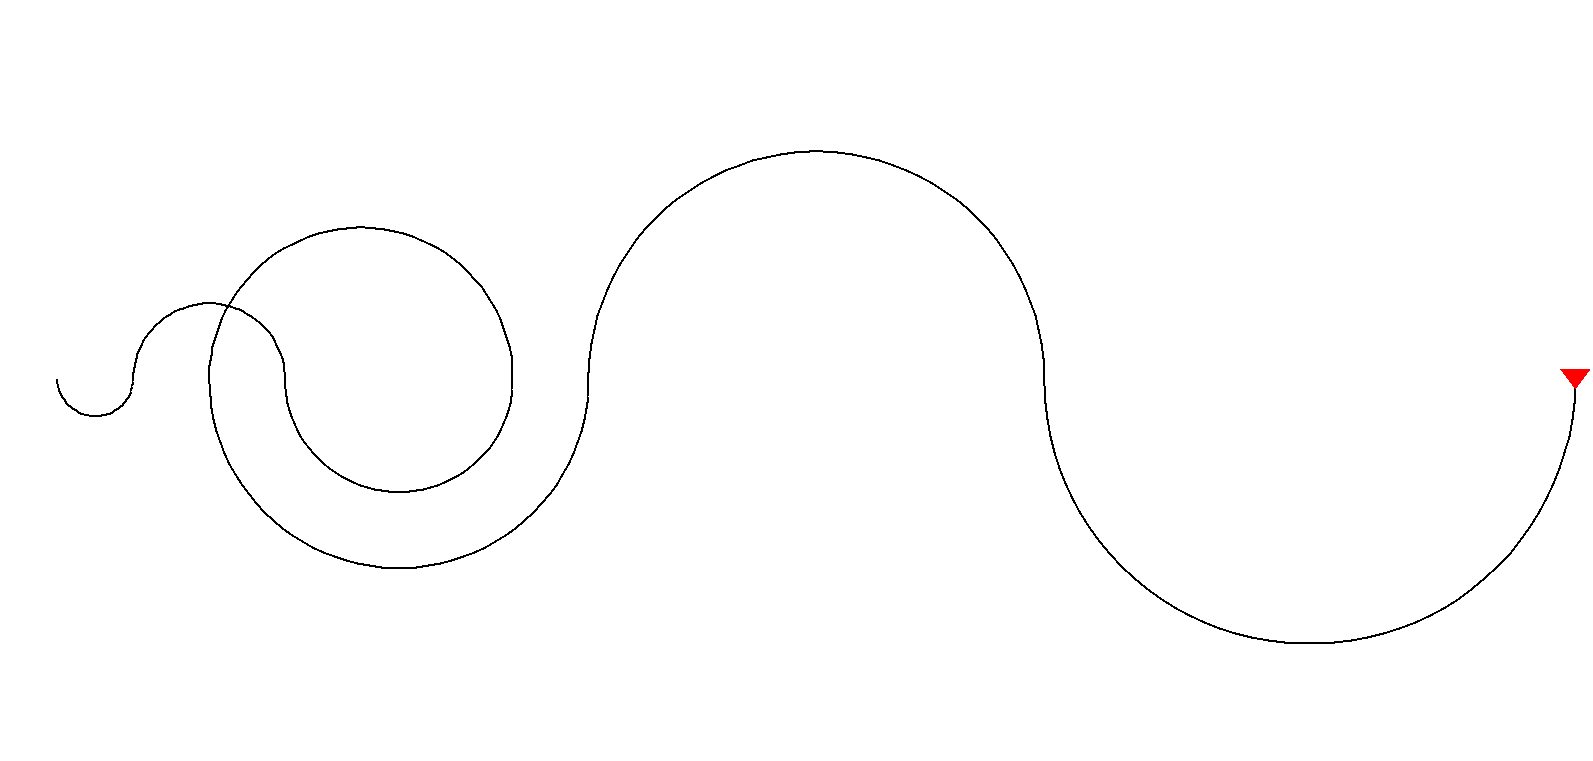
\includegraphics[width = \linewidth]{Sierpiński Arrowhead Curve/4.png}
		\caption{Iterate 4}
	\end{subfigure}
	\begin{subfigure}{0.18\linewidth}
		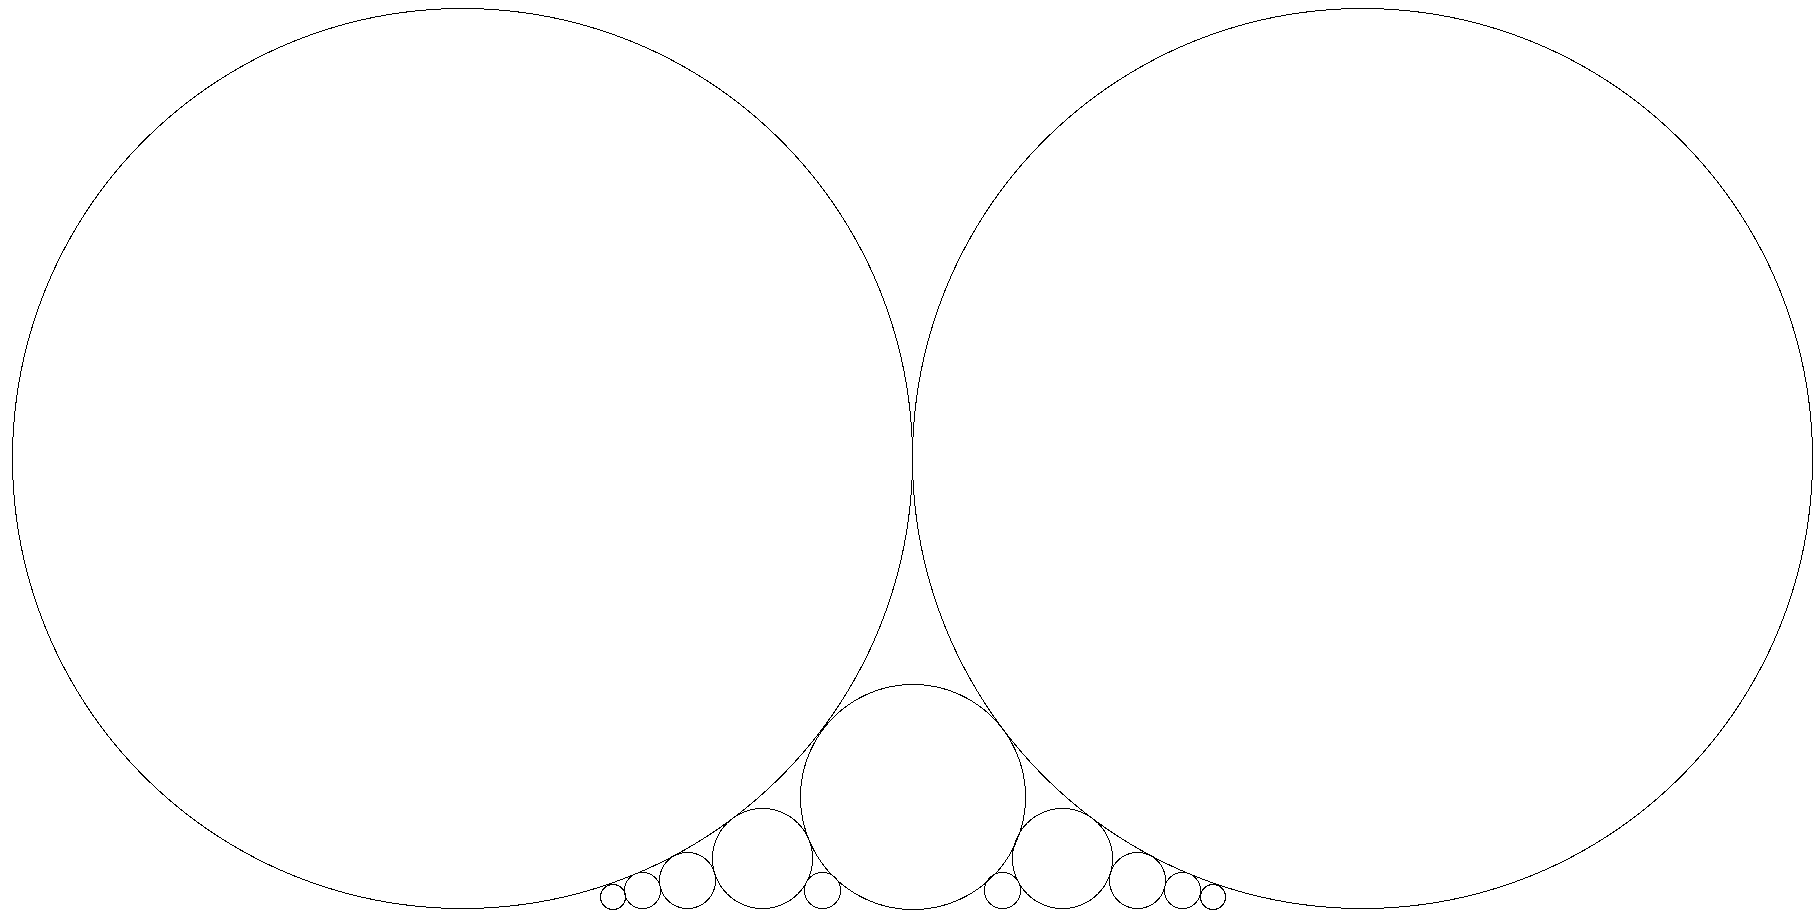
\includegraphics[width = \linewidth]{Sierpiński Arrowhead Curve/6.png}
		\caption{Iterate 6}
	\end{subfigure}
	\begin{subfigure}{0.18\linewidth}
		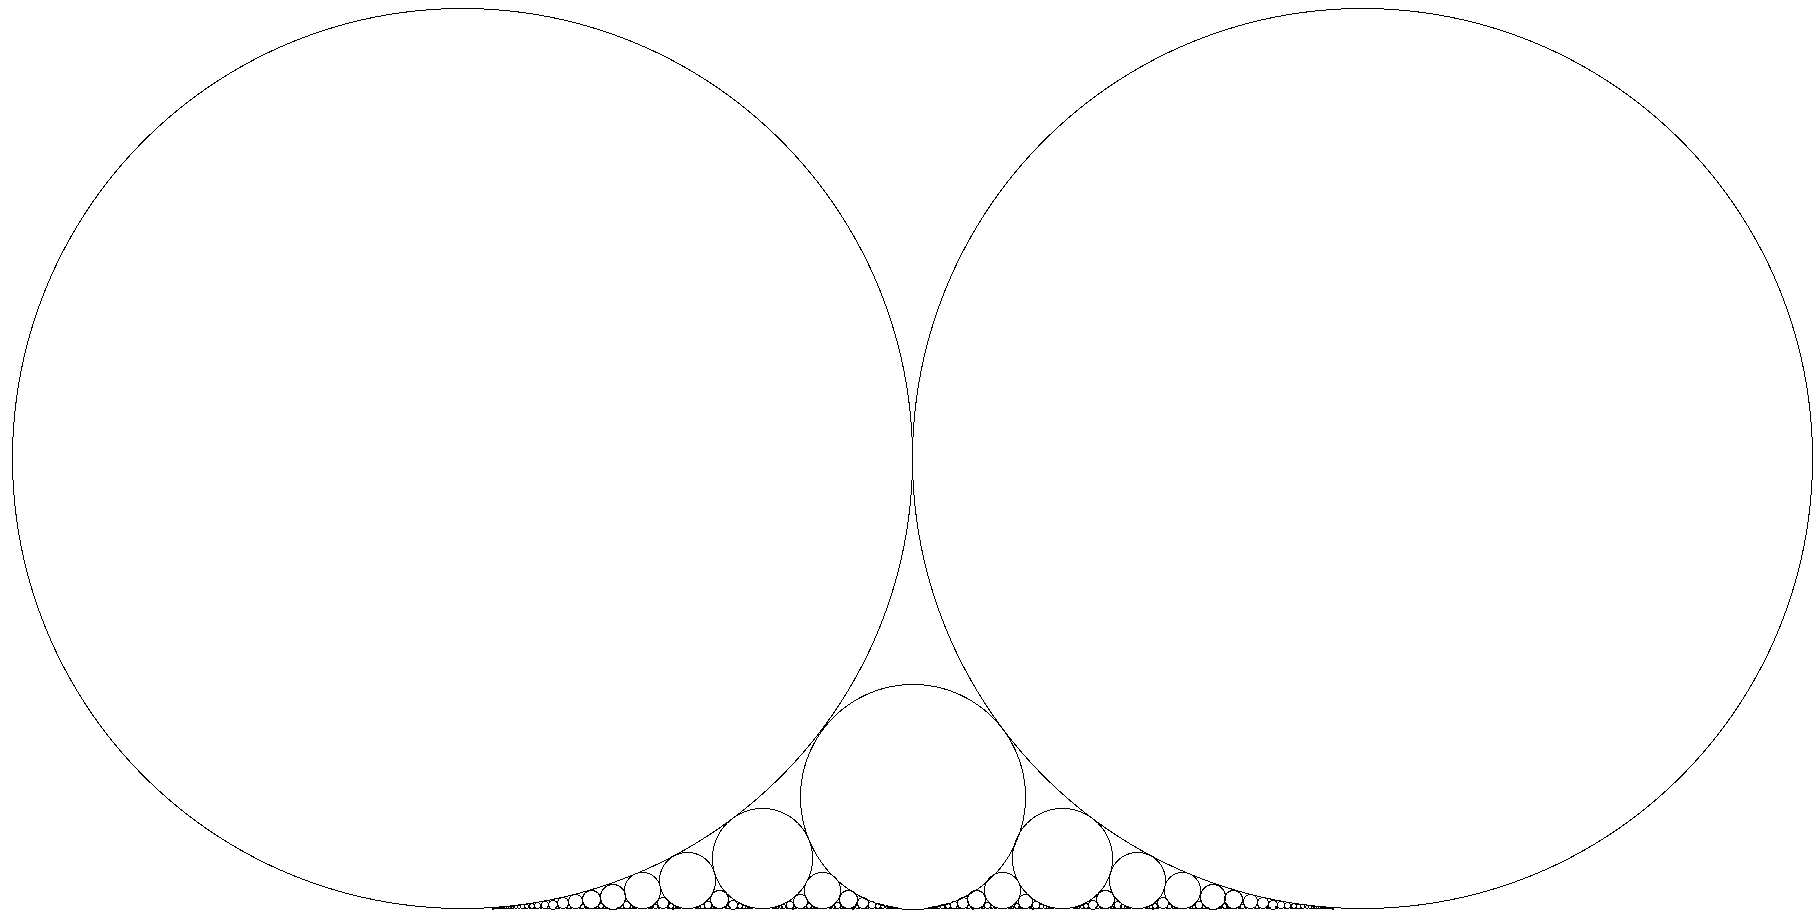
\includegraphics[width = \linewidth]{Sierpiński Arrowhead Curve/8.png}
		\caption{Iterate 8}
	\end{subfigure}
	\begin{subfigure}{0.18\linewidth}
		\includegraphics[width = \linewidth]{Sierpiński Arrowhead Curve/10.png}
		\caption{Iterate 10}
	\end{subfigure}
	\caption{Sierpi\'nski Arrowhead Curve for even iterates (why only even?)}
\end{figure}
\begin{funvideo}
	\href{https://youtu.be/UBuPWdSbyf8}{Unfolding The Dragon | Fractal Curve -- Think Twice}\\
	\href{https://youtu.be/gB9n2gHsHN4}{Fractals are typically not self-similar -- 3Blue1Brown}
\end{funvideo}
\end{document}